\documentclass[oneside,a4paper,11pt]{report}
%\usepackage[T1]{slovak}
\usepackage[utf8]{inputenc}
\usepackage{latexsym}
\usepackage{graphicx}
\usepackage{amsmath}
\usepackage{caption}
\usepackage{fancyhdr}
%\usepackage{picins}
\usepackage{times}
\usepackage{mathptmx}
\usepackage{url}
\usepackage{booktabs}
\usepackage{appendix}
\usepackage{rotating}
\usepackage{hyperref}
\pagestyle{fancy}
\fancyhead{}
\fancyhead[C]{\leftmark}
\renewcommand{\chaptermark}[1]{\markboth{\thechapter.\ #1}{}}


\usepackage[Sonny]{fncychap}
\makeatletter
 \ChNameVar{\small}
 \ChNumVar{\LARGE}
 \ChTitleVar{\LARGE\centering}
 \ChRuleWidth{0.05pt}
 \ChNameUpperCase

\usepackage{hyperref}
\newcommand\araa{ARA\&A}
\newcommand\aap{A\&A}

\usepackage{natbib}
% The astroads bibtex style formats the references according
% to the well-estabilished syntax in use in astronomy and
% creates a link if URLs are specified for a given record.

\bibliographystyle{astroads}


%\title{Štúdium premenných hviezd vo vysokoenergetickej části spektra}
\title{On stars in high energy }

\author{Matúš Kocka}



\begin{document}
%\begin{figure}
%\begin{center}
%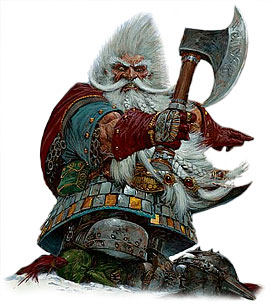
\includegraphics[width=6cm]{the-white-dwarf}
%\end{center}
%\end{figure}

\fancyhf{}
\newpage
\textit{"Per aspera ad astra..."}

\pagebreak
\tableofcontents

\addcontentsline{toc}{chapter}{\protect\numberline{}Introduction}
\chapter{Introduction to the stars in high energy }

Let your imagination soar. 
By sitting on the old rocker looking at the sky with couple of good old whiskey you can easily 
start thinking about the universe. You are looking at a heck of a different kinds of cosmic 
objects, but suddenly you see almost only the stars. Almost all the shiny dots on the sky are 
stars and these stars are only the closest ones. Yes, you can see few other 
galaxies by naked eye\footnote{M31 and M33 in extremely good conditions on northern hemisphere
and Magellanic clouds on southern one}, but none of the exotic cosmic objects you are imaging about. 
They are too faint to be observed easily, because they are not only far, far away, but also usually shines 
on different wavelengths, not visible by human eye.

Think about distances in the universe. One of the most accurate explanation is that from: \cite{hitch:1}  
\textit{"Space," it says, "is big. Really big. You just won't believe how vastly, 
hugely, mindbogglingly big it is. I mean, you may think it's a long way down the road to the 
chemist's, but that's just peanuts to space..."} 

Consider this, sometimes you want to study processes in these extreme, very faint objects, 
but they are too faint and too far in the universe. You are looking for “laboratory” with similar
 processes, but located mutch closer to the observer. The X-ray binary stars can be this kind 
of laboratories.  

There is, off-course, many interesting phenomena which could be studied in X-ray binaries or in non-binary X-ray stars. 
Several of them are mentioned in motivation section. 

I am mentioning many interesting thinks in this work, but main effort is taken to 
study post shock region in Intermediate Polars.   


\section{Motivation}
We easily find many reasons why to study stars in high energy bands.  
We can consider the direct and the most common scientific applications like observations of 
the supernovae, black holes \& neutron stars in X-ray binaries. But for education purposes 
I am preferring several others, very nice examples closer to topic of this work.  

\begin{itemize}
 \item \textbf{Relativistic jet phenomena}: like it was proposed by \citet{mirabel:1} that universal 
mechanism should be at work in all the relativistic jet sources in the universe. Better understanding 
of sources as: microblazars, AGNs and gamma-ray burst will helps to gain more comprehensive 
understanding of this phenomena. Microblazars can play role of “space laboratories”, where interesting
 processes last on different timescales as in the case with AGNs or GRBs.   

\begin{figure}[!hbt]
\centering
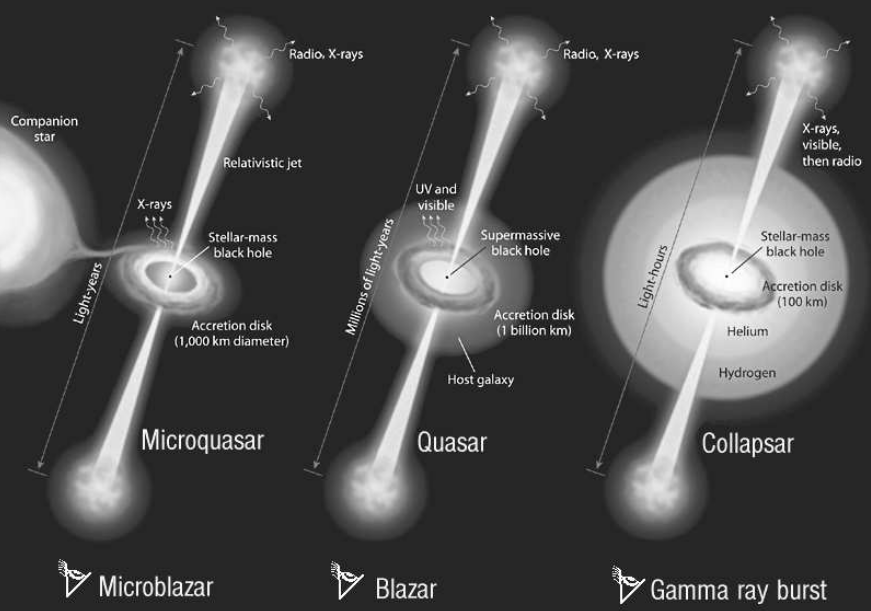
\includegraphics[totalheight=8.5cm]{microblazars}
\caption{NOT in scale diagram, showing curent ideas of micro-quasars, AGNs and gamma-ray
bursts as space objects driven by same, universal mechanism  \citet{mirabel:1}. }
\label{microblazar} 
\end{figure}

 \item \textbf{GXRE}: \citet{2007A&A...463..957K}

 \item \textbf{White dwarfs masses in IP}: \citet{2005A&A...435..191S}

\end{itemize}





\section{Observations}


\chapter{Cataclysmic variable stars}
\section{Non magnetic cataclysmic variables} 
\section{Magnetic cataclysmic variables}
\subsection{Polars}
\subsection{Intermediate polars}
\section{Galactic population ofcataclysmic variables }
\section{Others important creatures}
\section{GXRE}



\chapter{Model of post shock region}
\section{Thermal bremstalung}
\section{Post shock region}
\section{WD mass estimations methods}

\chapter{Data analysis}






%\section{Hmotnosť bieleho trpaslík}
%\subsection{Pomocou kontinua}
%\subsection{Pomocou K železných čiar}
%\chapter{Spracovanie dát}
%\section{INTEGRAL}
%\section{XMM-Newton}
%\chapter{Určenie hmotností vybraných IP}



%\chapter{Intermedialne polary}   


\nocite{2009A&A...496..121B}
\nocite{accpower:1}
\nocite{2005A&A...435..191S}
\nocite{2008A&A...489.1121R}
\nocite{2010A&A...520A..25Y}
\nocite{warner:1}
\nocite{2006A&A...450..117S}
\nocite{rybicki:1}
\nocite{1973PThPh..49.1184A_aizu}
\bibliography{koci}
\addcontentsline{toc}{chapter}{\hspace*{6mm}Bibliography}


%\begin{thebibliography}{99}
%\addcontentsline{toc}{chapter}{\hspace*{6mm}Literatúra}
%\bibitem {(Warner 1995)} B. Warner, 1995, Cataclysmic Variables, (Cambridge: Cambridge Univ. Press)
%\bibitem {(Rosswog 2007)} S. Rosswog, \& M. Br\"{u}ggen, 2007, Introduction to High-Energy Astrophysics,
%(Cambridge: Cambridge Univ. Press)
%\bibitem{(Douglas 1979)} A. Douglas, 1979, The Hitchhiker's Guide to the Galaxy, Pan Books,
%ISBN\,0330-25864-8 
%\bibitem[(Mirabel 2002)]{mirabel1} I. F. Mirabel, 2002, Microquasars as sources of high energy phenomena,
%arXiv:astro-ph/02110855 v1
%\end{thebibliography}



\clearpage

\appendix
\section*{Appendix}
\addcontentsline{toc}{chapter}{\hspace*{6mm}Apendix}
this will be the appendix
%\pagebreak



\begin{sidewaystable}
\begin{center}
 

\caption{Estimated WD masses from previous reports ...}
\begin{tabular}{llllllll}
\hline
\hline
%\multicolumn{2}{c}{Item} \\
System & Suzaku & Swift & RXTE & RXTE & Ginga & ASCA& This work  \\
       & XIS+HXD & BAT& PCA+HEXTE & PCA & LAC & SIS & XMM \& Integral                     \\
       & $M_{WD}$ &$M_{WD}$ &$M_{WD} $&$M_{WD}$ &$M_{WD}$ &$M_{WD}$ &$M_{WD}$ \\
\hline
 FO Aqr      &         &        &          &     &      &         &           \\
 XY Ari      &         &        &          &     &      &         &           \\
 MU Cam      &         &        &          &     &      &         &           \\
 BG CMi&         &        &          &     &      &         &           \\
 V709 Cas&         &        &          &     &      &         &           \\
 TV Col&         &        &          &     &      &         &           \\
 TX Col&         &        &          &     &      &         &           \\
 YY Dra&         &        &          &     &      &         &           \\
 PQ Gem&         &        &          &     &      &         &           \\
 EX Hya&         &        &          &     &      &         &           \\
 NY Lup&         &        &          &     &      &         &           \\
 V2400 Oph&         &        &          &     &      &         &           \\
 AO Psc&         &        &          &     &      &         &           \\
 V1223 Sgr&         &        &          &     &      &         &           \\
 RX J2133&         &        &          &     &      &         &           \\
 IGR J17303&         &        &          &     &      &         &           \\

\hline
\end{tabular}

\end{center}
\end{sidewaystable}
%\thispagestyle{empty}
%\LaTeX{}
\end{document}


